\subsubsection{3つのインストール方法}
Goにはいくつものインストール方法があります。どれでも好きなのを選んでかまいません。ここでは3つのよくあるインストール方法をご紹介します:

\begin{itemize}
  \item ソースコードのインストール:標準的なインストール方法です。Unix系システムをよく使うユーザ、特に開発者であれば、設定を好みに合わせて変更できます。
  \item 標準パッケージのインストール:Goは便利なインストールパッケージを用意しています。Windows, Linux, Macなどのシステムをサポートしています。とりあえずさっとインストールするにはうってつけでしょう。システムのbit数に対応したインストールパッケージをダウンロードして、"Next"をたどるだけでインストールできます。 \textbf{おすすめ}
  \item サードパーティツールによるインストール:現在便利なサードパーティパッケージも多くあります。たとえばUbuntuのapt-get、Macのhomebrewなどです。これらのシステムに慣れたユーザにはぴったりのインストール方法です。
\end{itemize}

最後に同じシステムの中で異なるバージョンのGoをインストールする場合は、GVM(https:\//\//github.com\//moovweb\//gvm)が参考になります。どうすればよいか分からない場合一番うまくやれます。

\subsubsection{Goソースコードのインストール}
GoのソースコードにはPlan 9 CとAT\&Tコンパイラを使って書かれている部分があります。もしソースコードからインストールしたい場合は、あらかじめCのコンパイルツールをインストールしておく必要があります。

Macでは、Xcodeに適切なコンパイラが含まれています。

Unixでは、gccなどのツールをインストールする必要があります。例えばUbuntuではターミナルで\texttt{sudo apt-get install gcc libc6-dev}を実行することでコンパイラをインストールすることができます。

Windowsでは、MinGWをインストールする必要があります。その後MinGWでgccをインストールして、適切な環境変数を設定します。

直接オフィシャルサイトからソースコードをダウンロードできます。対応する\texttt{goVERSION.src.tar.gz}のファイルをダウンロードし、\texttt{\$HOME}ディレクトリに解凍してから以下のコマンドを実行します。

\begin{lstlisting}[numbers=none]
cd go/src
./all.bash
\end{lstlisting}

all.bashを実行後"ALL TESTS PASSED"が表示されると、インストール成功です。

上記はUnixスタイルのコマンドです、Windowsもインストール方法は似ており、\texttt{all.bat}を実行するだけです。コンパイラはMinGWのgccを使います。

もしMacまたはUnixユーザであればいくつかの環境変数を設定する必要があります。再起動しても有効にしたい場合は以下のコマンドを\texttt{.bashrc}や\texttt{.zsh}に書いておきます。

\begin{lstlisting}[numbers=none]
export GOPATH=$HOME/gopath
export PATH=$PATH:$HOME/go/bin:$GOPATH/bin
\end{lstlisting}

ファイルに書き込んだ場合は、\texttt{bash .bashrc}や\texttt{bash .zshrc}を実行してすぐに設定を有効にします。

Windowsシステムの場合は、環境変数を設定する必要があります。pathにgoが存在するディレクトリを追加し、gopath変数を設定します。

設定が終わり、コマンドプロンプトで\texttt{go}を入力すると、下図のような画面が表示されるはずです。

\begin{figure}[H]
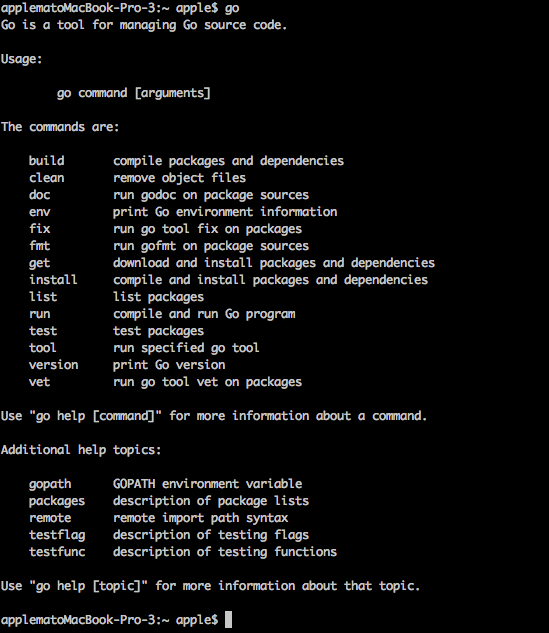
\includegraphics[width=14cm]{1.1.mac.png}
\label{図1.1}
\caption{ソースコードインストール後Goコマンドを実行}
\end{figure}

GoのUsage情報が表示されれば、Goのインストールは成功です:もしこのコマンドが存在しない場合は、PATH環境変数のなかにGoのインストールディレクトリが含まれているか確認してください。

\begin{quote}
  GOPATHについては以降の章で詳しくご説明します
\end{quote}




\subsubsection{Go標準パッケージのインストール}
Goはさまざまなプラットホームでインストールパッケージを提供しています、これらのパッケージはデフォルトで以下のディレクトリにインストールします:\//usr\//local\//go(Windows:c:$\backslash$ Go)。当然これらのインストール場所を変更することもできます、ただし変更後はあなたの環境変数を以下のように設定する必要があります:

\begin{lstlisting}[numbers=none]
export GOROOT=$HOME/go
export GOPATH=$HOME/gopath
export PATH=$PATH:$GOROOT/bin:$GOPATH/bin
\end{lstlisting}


これらのコマンドはMacやUnixユーザであれば\texttt{.bashrc}や\texttt{.zshrc}ファイルに入れておくべきでしょう。Windowsユーザであれば当然環境変数に入れておきます。

\subsubsection{自分の操作しているシステムが32bitか64bitか判断する方法}
Goのインストールにはオペレーティングシステムのbit数を判断する必要があるので、この章では先に自分のシステムの種類を確認しましょう。

WindowsのユーザはWin+Rを押してcmdを実行してください。\texttt{systeminfo}と入力してエンターキーを押します。しばらくするとシステムの情報が表示されます。"システムの種類"の一行に"x64-based PC"と表示されていれば64bitシステムです。もし"X86-based PC"とあれば、32bitシステムです。

Macユーザは直接64bit版を使用することをおすすめします。GoがサポートしているMac OS Xのバージョンは、すでに32bitプロセッサをサポートしていないためです。

LinuxユーザはTerminalで\texttt{arch}(すなわち、\texttt{uname -a})を実行することでシステムの情報を確かめることができます。

64bitシステムであれば以下のように表示されます。

\begin{lstlisting}[numbers=none]
x86_64
\end{lstlisting}

32bitシステムの場合は以下のように表示されます。

\begin{lstlisting}[numbers=none]
i386
\end{lstlisting}

\subsubsection{Mac インストール}
ダウンロードURLにアクセスし、32bitシステムはgo1.4.2.darwin-386-osx10.8.pkgをダウンロードします。64bitシステムであればgo1.4.2.darwin-amd64-osx10.8.pkgをダウンロードします。ファイルをダブルクリックし、すべてデフォルトで「次へ」ボタンをクリックします。これでgoはあなたのシステムにインストールされました。デフォルトでPATHの中に適切な\texttt{~\//go\//bin}が追加されています。端末を開いて\texttt{go}と入力します。

インストール成功の画像が表示されればインストール成功です。

もしgoのUsage情報が表示した場合は、goはすでにインストールされています。もしこのコマンドが存在しないと表示した場合は、自分のPATH環境変数の中にgoのインストールディレクトリが含まれているか確認してください。


\subsubsection{Linux インストール}
ダウンロードURLにアクセスし、32bitシステムであればgo1.4.2.linux-386.tar.gzを、64bitシステムであればgo1.2.2.linux-amd64.tar.gzをダウンロードします。

以下ではGoがインストールされたディレクトリを\texttt{\$GO\_INSTALL\_DIR}と仮定します。

\texttt{tar.gz}をインストールディレクトリに解凍します:\texttt{tar zxvf go1.4.2.linux-amd64.tar.gz -C \$GO\_INSTALL\_DIR}

PATHを設定します。\texttt{export PATH=\$PATH:\$GO\_INSTALL\_DIR\//go\//bin}

その後、\texttt{go}を実行します。

\begin{figure}[H]
  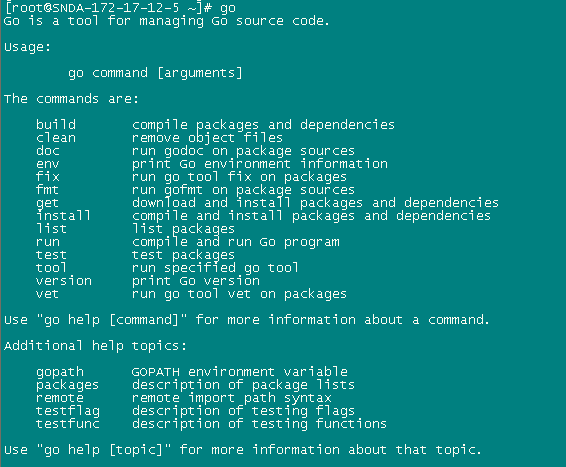
\includegraphics[width=14cm]{1.1.linux.png}
   \label{図1.2}
   \caption{Linuxシステムでインストールに成功したあとgoを実行した時に表示する情報}
\end{figure}

もしgoのUsage情報が表示された場合は、goはすでにインストールされています。もしこのコマンドが存在しないと出てきた場合は、自分のPATH環境変数の中にgoのインストールディレクトリが含まれているか確認してください。


\subsubsection{Windows インストール}
Google Code ダウンロードページ(http:\//\//golang.org\//dl\//)にアクセスし、32bit の場合は名前に windows-386 を含む msi パッケージを、64bit であれば名前に windows-amd64 を含むものをダウンロードします。ダウンロード後実行しますが、デフォルトのインストールフォルダである C:$\backslash$ Go$\backslash$を変更してはいけません。他の場所にインストールしてしまうと、あなたが書いた Go コードが実行できなくなってしまうかもしれません。インストールが終わるとデフォルトで環境変数 Path に Go のインストールフォルダの下にある bin フォルダ $C:\backslash Go\backslash bin\backslash$ が追加され、Go のインストールフォルダである $C:\backslash Go\backslash$ の値が環境変数 GOROOT に追加されます。

\paragraph{インストールが成功しているか確認する}


「ファイル名を指定して実行」に \texttt{cmd} を入力し、コマンドラインツールを開きます。プロンプトで\texttt{go}と入力することで Usage 情報が確認できるか確かめることができます。\texttt{cd \%GOROOT\%} を入力すると、Go のインストールフォルダに入れるか確認できます。どちらも成功していれば、インストールに成功しています。

インストールに成功していなければ、環境変数 Path と GOROOT の値を確認してください。もし存在しなければアンインストールの上再インストールし、存在していればコンピュータを再起動し、上の手順を再度試してください。


\subsubsection{サードパーティツールのインストール}
\paragraph{GVM}
gvmはサードパーティが開発したGoのバージョン管理ツールです。rubyのrvmツールに似ています。相当使い勝手がいいです。gvmをインストールするには以下のコマンド実行します:

\begin{lstlisting}[numbers=none]
bash < <(curl -s -S -L https://raw.github.com/moovweb
/gvm/master/binscripts/gvm-installer)
\end{lstlisting}

インストールが完了したあと、goをインストールすることができます:

\begin{lstlisting}[numbers=none]
gvm install go1.4.2
gvm use go1.4.2
\end{lstlisting}

下のコマンドで、毎回gvm useをコールする手間を省くことができます: gvm use go1.4.2 --default

上のコマンドを実行したあと、GOPATH、GOROOTなどの環境変数が自動的に設定されます。これで、直接利用することができます。

\paragraph{apt-get}
Ubuntuは現在最も多く利用されているLinuxデスクトップシステムです。\texttt{apt-get}コマンドでソフトウェア・パッケージを管理します。下のコマンドでGoをインストールすることができます、今後のため\texttt{git}と\texttt{mercurial}もインストールしておくべきでしょう:

\begin{lstlisting}[numbers=none]
sudo apt-get install python-software-properties
sudo add-apt-repository ppa:gophers/go
sudo apt-get update
sudo apt-get install golang-stable git-core mercurial
\end{lstlisting}

\paragraph{homebrew}
homebrewはMacで現在最も使用されているソフトウェア管理ツールです。現在Goをサポートしており、以下のコマンドでGoを直接インストールすることができます。今後のため\texttt{git}と\texttt{mercurial}もインストールしておくべきでしょう:

\begin{lstlisting}[numbers=none]
brew update && brew upgrade
brew install go
brew install git
brew install mercurial
\end{lstlisting}


